\documentclass[1p]{elsarticle_modified}
%\bibliographystyle{elsarticle-num}

%\usepackage[colorlinks]{hyperref}
%\usepackage{abbrmath_seonhwa} %\Abb, \Ascr, \Acal ,\Abf, \Afrak
\usepackage{amsfonts}
\usepackage{amssymb}
\usepackage{amsmath}
\usepackage{amsthm}
\usepackage{scalefnt}
\usepackage{amsbsy}
\usepackage{kotex}
\usepackage{caption}
\usepackage{subfig}
\usepackage{color}
\usepackage{graphicx}
\usepackage{xcolor} %% white, black, red, green, blue, cyan, magenta, yellow
\usepackage{float}
\usepackage{setspace}
\usepackage{hyperref}

\usepackage{tikz}
\usetikzlibrary{arrows}

\usepackage{multirow}
\usepackage{array} % fixed length table
\usepackage{hhline}

%%%%%%%%%%%%%%%%%%%%%
\makeatletter
\renewcommand*\env@matrix[1][\arraystretch]{%
	\edef\arraystretch{#1}%
	\hskip -\arraycolsep
	\let\@ifnextchar\new@ifnextchar
	\array{*\c@MaxMatrixCols c}}
\makeatother %https://tex.stackexchange.com/questions/14071/how-can-i-increase-the-line-spacing-in-a-matrix
%%%%%%%%%%%%%%%

\usepackage[normalem]{ulem}

\newcommand{\msout}[1]{\ifmmode\text{\sout{\ensuremath{#1}}}\else\sout{#1}\fi}
%SOURCE: \msout is \stkout macro in https://tex.stackexchange.com/questions/20609/strikeout-in-math-mode

\newcommand{\cancel}[1]{
	\ifmmode
	{\color{red}\msout{#1}}
	\else
	{\color{red}\sout{#1}}
	\fi
}

\newcommand{\add}[1]{
	{\color{blue}\uwave{#1}}
}

\newcommand{\replace}[2]{
	\ifmmode
	{\color{red}\msout{#1}}{\color{blue}\uwave{#2}}
	\else
	{\color{red}\sout{#1}}{\color{blue}\uwave{#2}}
	\fi
}

\newcommand{\Sol}{\mathcal{S}} %segment
\newcommand{\D}{D} %diagram
\newcommand{\A}{\mathcal{A}} %arc


%%%%%%%%%%%%%%%%%%%%%%%%%%%%%5 test

\def\sl{\operatorname{\textup{SL}}(2,\Cbb)}
\def\psl{\operatorname{\textup{PSL}}(2,\Cbb)}
\def\quan{\mkern 1mu \triangleright \mkern 1mu}

\theoremstyle{definition}
\newtheorem{thm}{Theorem}[section]
\newtheorem{prop}[thm]{Proposition}
\newtheorem{lem}[thm]{Lemma}
\newtheorem{ques}[thm]{Question}
\newtheorem{cor}[thm]{Corollary}
\newtheorem{defn}[thm]{Definition}
\newtheorem{exam}[thm]{Example}
\newtheorem{rmk}[thm]{Remark}
\newtheorem{alg}[thm]{Algorithm}

\newcommand{\I}{\sqrt{-1}}
\begin{document}

%\begin{frontmatter}
%
%\title{Boundary parabolic representations of knots up to 8 crossings}
%
%%% Group authors per affiliation:
%\author{Yunhi Cho} 
%\address{Department of Mathematics, University of Seoul, Seoul, Korea}
%\ead{yhcho@uos.ac.kr}
%
%
%\author{Seonhwa Kim} %\fnref{s_kim}}
%\address{Center for Geometry and Physics, Institute for Basic Science, Pohang, 37673, Korea}
%\ead{ryeona17@ibs.re.kr}
%
%\author{Hyuk Kim}
%\address{Department of Mathematical Sciences, Seoul National University, Seoul 08826, Korea}
%\ead{hyukkim@snu.ac.kr}
%
%\author{Seokbeom Yoon}
%\address{Department of Mathematical Sciences, Seoul National University, Seoul, 08826,  Korea}
%\ead{sbyoon15@snu.ac.kr}
%
%\begin{abstract}
%We find all boundary parabolic representation of knots up to 8 crossings.
%
%\end{abstract}
%\begin{keyword}
%    \MSC[2010] 57M25 
%\end{keyword}
%
%\end{frontmatter}

%\linenumbers
%\tableofcontents
%
\newcommand\colored[1]{\textcolor{white}{\rule[-0.35ex]{0.8em}{1.4ex}}\kern-0.8em\color{red} #1}%
%\newcommand\colored[1]{\textcolor{white}{ #1}\kern-2.17ex	\textcolor{white}{ #1}\kern-1.81ex	\textcolor{white}{ #1}\kern-2.15ex\color{red}#1	}

{\Large $\underline{12a_{0063}~(K12a_{0063})}$}

\setlength{\tabcolsep}{10pt}
\renewcommand{\arraystretch}{1.6}
\vspace{1cm}\begin{tabular}{m{100pt}>{\centering\arraybackslash}m{274pt}}
\multirow{5}{120pt}{
	\centering
	\includegraphics[width=112pt]{../../../GIT/diagram.site/Diagrams/png/864_12a_0063.png}\\
\ \ \ A knot diagram\footnotemark}&
\allowdisplaybreaks
\textbf{Linearized knot diagam} \\
\cline{2-2}
 &
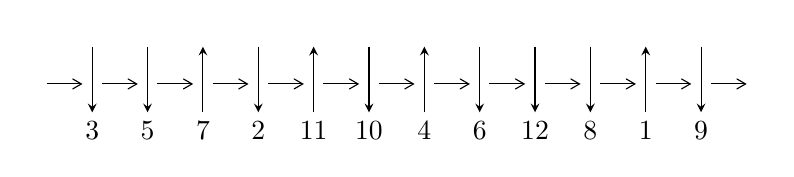
\begin{tikzpicture}[x=20pt, y=17pt]
	% nodes
	\node (C0) at (0, 0) {};
	\node (C1) at (1, 0) {};
	\node (C1U) at (1, +1) {};
	\node (C1D) at (1, -1) {3};

	\node (C2) at (2, 0) {};
	\node (C2U) at (2, +1) {};
	\node (C2D) at (2, -1) {5};

	\node (C3) at (3, 0) {};
	\node (C3U) at (3, +1) {};
	\node (C3D) at (3, -1) {7};

	\node (C4) at (4, 0) {};
	\node (C4U) at (4, +1) {};
	\node (C4D) at (4, -1) {2};

	\node (C5) at (5, 0) {};
	\node (C5U) at (5, +1) {};
	\node (C5D) at (5, -1) {11};

	\node (C6) at (6, 0) {};
	\node (C6U) at (6, +1) {};
	\node (C6D) at (6, -1) {10};

	\node (C7) at (7, 0) {};
	\node (C7U) at (7, +1) {};
	\node (C7D) at (7, -1) {4};

	\node (C8) at (8, 0) {};
	\node (C8U) at (8, +1) {};
	\node (C8D) at (8, -1) {6};

	\node (C9) at (9, 0) {};
	\node (C9U) at (9, +1) {};
	\node (C9D) at (9, -1) {12};

	\node (C10) at (10, 0) {};
	\node (C10U) at (10, +1) {};
	\node (C10D) at (10, -1) {8};

	\node (C11) at (11, 0) {};
	\node (C11U) at (11, +1) {};
	\node (C11D) at (11, -1) {1};

	\node (C12) at (12, 0) {};
	\node (C12U) at (12, +1) {};
	\node (C12D) at (12, -1) {9};
	\node (C13) at (13, 0) {};

	% arrows
	\draw[->,>={angle 60}]
	(C0) edge (C1) (C1) edge (C2) (C2) edge (C3) (C3) edge (C4) (C4) edge (C5) (C5) edge (C6) (C6) edge (C7) (C7) edge (C8) (C8) edge (C9) (C9) edge (C10) (C10) edge (C11) (C11) edge (C12) (C12) edge (C13) ;	\draw[->,>=stealth]
	(C1U) edge (C1D) (C2U) edge (C2D) (C3D) edge (C3U) (C4U) edge (C4D) (C5D) edge (C5U) (C6U) edge (C6D) (C7D) edge (C7U) (C8U) edge (C8D) (C9U) edge (C9D) (C10U) edge (C10D) (C11D) edge (C11U) (C12U) edge (C12D) ;
	\end{tikzpicture} \\
\hhline{~~} \\& 
\textbf{Solving Sequence} \\ \cline{2-2} 
 &
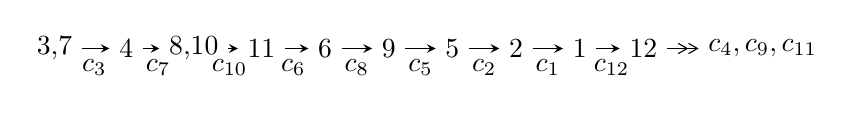
\begin{tikzpicture}[x=23pt, y=7pt]
	% node
	\node (A0) at (-1/8, 0) {3,7};
	\node (A1) at (1, 0) {4};
	\node (A2) at (33/16, 0) {8,10};
	\node (A3) at (25/8, 0) {11};
	\node (A4) at (33/8, 0) {6};
	\node (A5) at (41/8, 0) {9};
	\node (A6) at (49/8, 0) {5};
	\node (A7) at (57/8, 0) {2};
	\node (A8) at (65/8, 0) {1};
	\node (A9) at (73/8, 0) {12};
	\node (C1) at (1/2, -1) {$c_{3}$};
	\node (C2) at (3/2, -1) {$c_{7}$};
	\node (C3) at (21/8, -1) {$c_{10}$};
	\node (C4) at (29/8, -1) {$c_{6}$};
	\node (C5) at (37/8, -1) {$c_{8}$};
	\node (C6) at (45/8, -1) {$c_{5}$};
	\node (C7) at (53/8, -1) {$c_{2}$};
	\node (C8) at (61/8, -1) {$c_{1}$};
	\node (C9) at (69/8, -1) {$c_{12}$};
	\node (A10) at (11, 0) {$c_{4},c_{9},c_{11}$};

	% edge
	\draw[->,>=stealth]	
	(A0) edge (A1) (A1) edge (A2) (A2) edge (A3) (A3) edge (A4) (A4) edge (A5) (A5) edge (A6) (A6) edge (A7) (A7) edge (A8) (A8) edge (A9) ;
	\draw[->>,>={angle 60}]	
	(A9) edge (A10);
\end{tikzpicture} \\ 

\end{tabular} \\

\footnotetext{
The image of knot diagram is generated by the software ``\textbf{Draw programme}" developed by Andrew Bartholomew(\url{http://www.layer8.co.uk/maths/draw/index.htm\#Running-draw}), where we modified some parts for our purpose(\url{https://github.com/CATsTAILs/LinksPainter}).
}\phantom \\ \newline 
\centering \textbf{Ideals for irreducible components\footnotemark of $X_{\text{par}}$} 
 
\begin{align*}
I^u_{1}&=\langle 
4.30388\times10^{564} u^{137}+5.80260\times10^{564} u^{136}+\cdots+2.13528\times10^{566} b-8.99538\times10^{567},\\
\phantom{I^u_{1}}&\phantom{= \langle  }1.61908\times10^{565} u^{137}+2.38731\times10^{565} u^{136}+\cdots+1.70823\times10^{566} a-2.06670\times10^{568},\\
\phantom{I^u_{1}}&\phantom{= \langle  }u^{138}+u^{137}+\cdots-4096 u+512\rangle \\
\\
I^v_{1}&=\langle 
a,\;-117084 v^8-101146 v^7+\cdots+178147 b-213819,\\
\phantom{I^v_{1}}&\phantom{= \langle  }v^9+v^8+12 v^7+7 v^6+37 v^5- v^4+10 v^2+5 v+1\rangle \\
\end{align*}
\raggedright * 2 irreducible components of $\dim_{\mathbb{C}}=0$, with total 147 representations.\\
\footnotetext{All coefficients of polynomials are rational numbers. But the coefficients are sometimes approximated in decimal forms when there is not enough margin.}
\newpage
\renewcommand{\arraystretch}{1}
\centering \section*{I. $I^u_{1}= \langle 4.30\times10^{564} u^{137}+5.80\times10^{564} u^{136}+\cdots+2.14\times10^{566} b-9.00\times10^{567},\;1.62\times10^{565} u^{137}+2.39\times10^{565} u^{136}+\cdots+1.71\times10^{566} a-2.07\times10^{568},\;u^{138}+u^{137}+\cdots-4096 u+512 \rangle$}
\flushleft \textbf{(i) Arc colorings}\\
\begin{tabular}{m{7pt} m{180pt} m{7pt} m{180pt} }
\flushright $a_{3}=$&$\begin{pmatrix}1\\0\end{pmatrix}$ \\
\flushright $a_{7}=$&$\begin{pmatrix}0\\u\end{pmatrix}$ \\
\flushright $a_{4}=$&$\begin{pmatrix}1\\- u^2\end{pmatrix}$ \\
\flushright $a_{8}=$&$\begin{pmatrix}u\\- u^3+u\end{pmatrix}$ \\
\flushright $a_{10}=$&$\begin{pmatrix}-0.0947815 u^{137}-0.139754 u^{136}+\cdots-690.527 u+120.985\\-0.0201560 u^{137}-0.0271749 u^{136}+\cdots-205.406 u+42.1274\end{pmatrix}$ \\
\flushright $a_{11}=$&$\begin{pmatrix}-0.109900 u^{137}-0.159663 u^{136}+\cdots-771.989 u+134.827\\-0.0307500 u^{137}-0.0424307 u^{136}+\cdots-274.982 u+53.5163\end{pmatrix}$ \\
\flushright $a_{6}=$&$\begin{pmatrix}-0.0831024 u^{137}-0.108477 u^{136}+\cdots-560.659 u+98.6070\\-0.00173320 u^{137}+0.00661599 u^{136}+\cdots-97.7944 u+16.3916\end{pmatrix}$ \\
\flushright $a_{9}=$&$\begin{pmatrix}0.0725287 u^{137}+0.102880 u^{136}+\cdots+471.818 u-81.4870\\0.0438673 u^{137}+0.0591812 u^{136}+\cdots+293.028 u-50.0935\end{pmatrix}$ \\
\flushright $a_{5}=$&$\begin{pmatrix}-0.0330916 u^{137}-0.0487965 u^{136}+\cdots-201.962 u+34.3636\\0.0474245 u^{137}+0.0709201 u^{136}+\cdots+317.724 u-51.4355\end{pmatrix}$ \\
\flushright $a_{2}=$&$\begin{pmatrix}-0.0330916 u^{137}-0.0487965 u^{136}+\cdots-201.962 u+34.3636\\-0.0405873 u^{137}-0.0610350 u^{136}+\cdots-270.340 u+43.3946\end{pmatrix}$ \\
\flushright $a_{1}=$&$\begin{pmatrix}-0.0736789 u^{137}-0.109832 u^{136}+\cdots-472.302 u+77.7582\\-0.0405873 u^{137}-0.0610350 u^{136}+\cdots-270.340 u+43.3946\end{pmatrix}$ \\
\flushright $a_{12}=$&$\begin{pmatrix}-0.0908434 u^{137}-0.134176 u^{136}+\cdots-634.531 u+110.010\\-0.0349893 u^{137}-0.0500330 u^{136}+\cdots-305.131 u+55.1204\end{pmatrix}$\\&\end{tabular}
\flushleft \textbf{(ii) Obstruction class $= -1$}\\~\\
\flushleft \textbf{(iii) Cusp Shapes $= 0.544581 u^{137}+0.814468 u^{136}+\cdots+3277.04 u-506.995$}\\~\\
\newpage\renewcommand{\arraystretch}{1}
\flushleft \textbf{(iv) u-Polynomials at the component}\newline \\
\begin{tabular}{m{50pt}|m{274pt}}
Crossings & \hspace{64pt}u-Polynomials at each crossing \\
\hline $$\begin{aligned}c_{1}\end{aligned}$$&$\begin{aligned}
&u^{138}+70 u^{137}+\cdots-82 u+1
\end{aligned}$\\
\hline $$\begin{aligned}c_{2},c_{4}\end{aligned}$$&$\begin{aligned}
&u^{138}-10 u^{137}+\cdots+14 u-1
\end{aligned}$\\
\hline $$\begin{aligned}c_{3},c_{7}\end{aligned}$$&$\begin{aligned}
&u^{138}- u^{137}+\cdots+4096 u+512
\end{aligned}$\\
\hline $$\begin{aligned}c_{5}\end{aligned}$$&$\begin{aligned}
&u^{138}+6 u^{137}+\cdots-67104 u-2117
\end{aligned}$\\
\hline $$\begin{aligned}c_{6}\end{aligned}$$&$\begin{aligned}
&u^{138}+2 u^{137}+\cdots-2626 u-97
\end{aligned}$\\
\hline $$\begin{aligned}c_{8}\end{aligned}$$&$\begin{aligned}
&u^{138}-10 u^{137}+\cdots+2 u-1
\end{aligned}$\\
\hline $$\begin{aligned}c_{9},c_{12}\end{aligned}$$&$\begin{aligned}
&u^{138}-2 u^{137}+\cdots+14 u+1
\end{aligned}$\\
\hline $$\begin{aligned}c_{10}\end{aligned}$$&$\begin{aligned}
&u^{138}-14 u^{137}+\cdots-2 u+1
\end{aligned}$\\
\hline $$\begin{aligned}c_{11}\end{aligned}$$&$\begin{aligned}
&u^{138}-54 u^{137}+\cdots+14 u+1
\end{aligned}$\\
\hline
\end{tabular}\\~\\
\newpage\renewcommand{\arraystretch}{1}
\flushleft \textbf{(v) Riley Polynomials at the component}\newline \\
\begin{tabular}{m{50pt}|m{274pt}}
Crossings & \hspace{64pt}Riley Polynomials at each crossing \\
\hline $$\begin{aligned}c_{1}\end{aligned}$$&$\begin{aligned}
&y^{138}+6 y^{137}+\cdots-5018 y+1
\end{aligned}$\\
\hline $$\begin{aligned}c_{2},c_{4}\end{aligned}$$&$\begin{aligned}
&y^{138}-70 y^{137}+\cdots+82 y+1
\end{aligned}$\\
\hline $$\begin{aligned}c_{3},c_{7}\end{aligned}$$&$\begin{aligned}
&y^{138}-57 y^{137}+\cdots-8912896 y+262144
\end{aligned}$\\
\hline $$\begin{aligned}c_{5}\end{aligned}$$&$\begin{aligned}
&y^{138}-118 y^{137}+\cdots-1356064422 y+4481689
\end{aligned}$\\
\hline $$\begin{aligned}c_{6}\end{aligned}$$&$\begin{aligned}
&y^{138}-166 y^{137}+\cdots+9748742 y+9409
\end{aligned}$\\
\hline $$\begin{aligned}c_{8}\end{aligned}$$&$\begin{aligned}
&y^{138}-14 y^{137}+\cdots-10 y+1
\end{aligned}$\\
\hline $$\begin{aligned}c_{9},c_{12}\end{aligned}$$&$\begin{aligned}
&y^{138}+54 y^{137}+\cdots-14 y+1
\end{aligned}$\\
\hline $$\begin{aligned}c_{10}\end{aligned}$$&$\begin{aligned}
&y^{138}-10 y^{137}+\cdots-14 y+1
\end{aligned}$\\
\hline $$\begin{aligned}c_{11}\end{aligned}$$&$\begin{aligned}
&y^{138}+62 y^{137}+\cdots+2378 y+1
\end{aligned}$\\
\hline
\end{tabular}\\~\\
\newpage\flushleft \textbf{(vi) Complex Volumes and Cusp Shapes}
$$\begin{array}{c|c|c}  
\text{Solutions to }I^u_{1}& \I (\text{vol} + \sqrt{-1}CS) & \text{Cusp shape}\\
 \hline 
\begin{aligned}
u &= \phantom{-}0.891237 + 0.451061 I \\
a &= -0.373810 + 0.420098 I \\
b &= \phantom{-}0.10213 + 2.17730 I\end{aligned}
 & -1.21505 + 3.56819 I & \phantom{-0.000000 } 0 \\ \hline\begin{aligned}
u &= \phantom{-}0.891237 - 0.451061 I \\
a &= -0.373810 - 0.420098 I \\
b &= \phantom{-}0.10213 - 2.17730 I\end{aligned}
 & -1.21505 - 3.56819 I & \phantom{-0.000000 } 0 \\ \hline\begin{aligned}
u &= \phantom{-}1.002230 + 0.056995 I \\
a &= -0.978568 - 0.559753 I \\
b &= \phantom{-}1.40585 - 0.25622 I\end{aligned}
 & \phantom{-}2.60318 - 4.38929 I & \phantom{-0.000000 } 0 \\ \hline\begin{aligned}
u &= \phantom{-}1.002230 - 0.056995 I \\
a &= -0.978568 + 0.559753 I \\
b &= \phantom{-}1.40585 + 0.25622 I\end{aligned}
 & \phantom{-}2.60318 + 4.38929 I & \phantom{-0.000000 } 0 \\ \hline\begin{aligned}
u &= -0.535602 + 0.829305 I \\
a &= -0.579407 - 0.422359 I \\
b &= -0.03823 - 2.72025 I\end{aligned}
 & -2.92258 + 5.51420 I & \phantom{-0.000000 } 0 \\ \hline\begin{aligned}
u &= -0.535602 - 0.829305 I \\
a &= -0.579407 + 0.422359 I \\
b &= -0.03823 + 2.72025 I\end{aligned}
 & -2.92258 - 5.51420 I & \phantom{-0.000000 } 0 \\ \hline\begin{aligned}
u &= -0.607911 + 0.752609 I \\
a &= -0.586692 - 0.433371 I \\
b &= \phantom{-}1.38290 - 0.95935 I\end{aligned}
 & -4.92549 + 2.89963 I & \phantom{-0.000000 } 0 \\ \hline\begin{aligned}
u &= -0.607911 - 0.752609 I \\
a &= -0.586692 + 0.433371 I \\
b &= \phantom{-}1.38290 + 0.95935 I\end{aligned}
 & -4.92549 - 2.89963 I & \phantom{-0.000000 } 0 \\ \hline\begin{aligned}
u &= -0.856902 + 0.439878 I \\
a &= \phantom{-}0.776533 - 0.191475 I \\
b &= \phantom{-}0.248146 - 0.070340 I\end{aligned}
 & \phantom{-}1.42734 - 1.67105 I & \phantom{-0.000000 } 0 \\ \hline\begin{aligned}
u &= -0.856902 - 0.439878 I \\
a &= \phantom{-}0.776533 + 0.191475 I \\
b &= \phantom{-}0.248146 + 0.070340 I\end{aligned}
 & \phantom{-}1.42734 + 1.67105 I & \phantom{-0.000000 } 0\\
 \hline 
 \end{array}$$\newpage$$\begin{array}{c|c|c}  
\text{Solutions to }I^u_{1}& \I (\text{vol} + \sqrt{-1}CS) & \text{Cusp shape}\\
 \hline 
\begin{aligned}
u &= \phantom{-}0.399102 + 0.957238 I \\
a &= \phantom{-}1.047610 - 0.663365 I \\
b &= \phantom{-}0.23151 - 1.43448 I\end{aligned}
 & -2.80156 - 2.93042 I & \phantom{-0.000000 } 0 \\ \hline\begin{aligned}
u &= \phantom{-}0.399102 - 0.957238 I \\
a &= \phantom{-}1.047610 + 0.663365 I \\
b &= \phantom{-}0.23151 + 1.43448 I\end{aligned}
 & -2.80156 + 2.93042 I & \phantom{-0.000000 } 0 \\ \hline\begin{aligned}
u &= -0.901914 + 0.317542 I \\
a &= \phantom{-}2.35366 + 0.86813 I \\
b &= -0.25586 + 1.95557 I\end{aligned}
 & \phantom{-}1.38659 + 0.85768 I & \phantom{-0.000000 } 0 \\ \hline\begin{aligned}
u &= -0.901914 - 0.317542 I \\
a &= \phantom{-}2.35366 - 0.86813 I \\
b &= -0.25586 - 1.95557 I\end{aligned}
 & \phantom{-}1.38659 - 0.85768 I & \phantom{-0.000000 } 0 \\ \hline\begin{aligned}
u &= -0.643323 + 0.685004 I \\
a &= \phantom{-}0.437804 + 0.707830 I \\
b &= -0.04627 + 2.82885 I\end{aligned}
 & -5.01384 - 0.52036 I & \phantom{-0.000000 } 0 \\ \hline\begin{aligned}
u &= -0.643323 - 0.685004 I \\
a &= \phantom{-}0.437804 - 0.707830 I \\
b &= -0.04627 - 2.82885 I\end{aligned}
 & -5.01384 + 0.52036 I & \phantom{-0.000000 } 0 \\ \hline\begin{aligned}
u &= -1.042910 + 0.202388 I \\
a &= -2.42701 - 0.42060 I \\
b &= \phantom{-}0.837030 - 0.935034 I\end{aligned}
 & \phantom{-}2.43266 + 1.40735 I & \phantom{-0.000000 } 0 \\ \hline\begin{aligned}
u &= -1.042910 - 0.202388 I \\
a &= -2.42701 + 0.42060 I \\
b &= \phantom{-}0.837030 + 0.935034 I\end{aligned}
 & \phantom{-}2.43266 - 1.40735 I & \phantom{-0.000000 } 0 \\ \hline\begin{aligned}
u &= -0.447071 + 0.969480 I \\
a &= \phantom{-}1.042050 + 0.194188 I \\
b &= \phantom{-}0.357165 + 0.646159 I\end{aligned}
 & \phantom{-}1.61097 + 5.54766 I & \phantom{-0.000000 } 0 \\ \hline\begin{aligned}
u &= -0.447071 - 0.969480 I \\
a &= \phantom{-}1.042050 - 0.194188 I \\
b &= \phantom{-}0.357165 - 0.646159 I\end{aligned}
 & \phantom{-}1.61097 - 5.54766 I & \phantom{-0.000000 } 0\\
 \hline 
 \end{array}$$\newpage$$\begin{array}{c|c|c}  
\text{Solutions to }I^u_{1}& \I (\text{vol} + \sqrt{-1}CS) & \text{Cusp shape}\\
 \hline 
\begin{aligned}
u &= -0.983568 + 0.420621 I \\
a &= \phantom{-}1.125930 - 0.299292 I \\
b &= -0.980929 + 0.486896 I\end{aligned}
 & \phantom{-}1.52583 + 0.05279 I & \phantom{-0.000000 } 0 \\ \hline\begin{aligned}
u &= -0.983568 - 0.420621 I \\
a &= \phantom{-}1.125930 + 0.299292 I \\
b &= -0.980929 - 0.486896 I\end{aligned}
 & \phantom{-}1.52583 - 0.05279 I & \phantom{-0.000000 } 0 \\ \hline\begin{aligned}
u &= -1.007240 + 0.365828 I \\
a &= -2.94257 - 0.96802 I \\
b &= \phantom{-}0.78500 - 2.45396 I\end{aligned}
 & \phantom{-}1.86133 - 3.37943 I & \phantom{-0.000000 } 0 \\ \hline\begin{aligned}
u &= -1.007240 - 0.365828 I \\
a &= -2.94257 + 0.96802 I \\
b &= \phantom{-}0.78500 + 2.45396 I\end{aligned}
 & \phantom{-}1.86133 + 3.37943 I & \phantom{-0.000000 } 0 \\ \hline\begin{aligned}
u &= \phantom{-}0.562307 + 0.712073 I \\
a &= -0.467713 - 0.587197 I \\
b &= -0.682448 - 0.564071 I\end{aligned}
 & -2.24121 - 1.11087 I & \phantom{-0.000000 } 0 \\ \hline\begin{aligned}
u &= \phantom{-}0.562307 - 0.712073 I \\
a &= -0.467713 + 0.587197 I \\
b &= -0.682448 + 0.564071 I\end{aligned}
 & -2.24121 + 1.11087 I & \phantom{-0.000000 } 0 \\ \hline\begin{aligned}
u &= \phantom{-}0.049286 + 0.900920 I \\
a &= -0.852074 + 0.482128 I \\
b &= -0.437779 + 0.125177 I\end{aligned}
 & \phantom{-}2.85912 - 1.44732 I & \phantom{-0.000000 } 0 \\ \hline\begin{aligned}
u &= \phantom{-}0.049286 - 0.900920 I \\
a &= -0.852074 - 0.482128 I \\
b &= -0.437779 - 0.125177 I\end{aligned}
 & \phantom{-}2.85912 + 1.44732 I & \phantom{-0.000000 } 0 \\ \hline\begin{aligned}
u &= \phantom{-}1.013460 + 0.467152 I \\
a &= -0.566480 + 0.532942 I \\
b &= \phantom{-}1.96084 + 1.00994 I\end{aligned}
 & \phantom{-}1.14019 + 6.08874 I & \phantom{-0.000000 } 0 \\ \hline\begin{aligned}
u &= \phantom{-}1.013460 - 0.467152 I \\
a &= -0.566480 - 0.532942 I \\
b &= \phantom{-}1.96084 - 1.00994 I\end{aligned}
 & \phantom{-}1.14019 - 6.08874 I & \phantom{-0.000000 } 0\\
 \hline 
 \end{array}$$\newpage$$\begin{array}{c|c|c}  
\text{Solutions to }I^u_{1}& \I (\text{vol} + \sqrt{-1}CS) & \text{Cusp shape}\\
 \hline 
\begin{aligned}
u &= -0.821216 + 0.326395 I \\
a &= -0.333026 - 1.123350 I \\
b &= -0.26649 - 1.98988 I\end{aligned}
 & \phantom{-}0.77318 - 3.15109 I & \phantom{-0.000000 } 0 \\ \hline\begin{aligned}
u &= -0.821216 - 0.326395 I \\
a &= -0.333026 + 1.123350 I \\
b &= -0.26649 + 1.98988 I\end{aligned}
 & \phantom{-}0.77318 + 3.15109 I & \phantom{-0.000000 } 0 \\ \hline\begin{aligned}
u &= -0.974643 + 0.546694 I \\
a &= \phantom{-}0.543194 + 1.122300 I \\
b &= -0.58768 + 2.16848 I\end{aligned}
 & -5.66343 - 4.80751 I & \phantom{-0.000000 } 0 \\ \hline\begin{aligned}
u &= -0.974643 - 0.546694 I \\
a &= \phantom{-}0.543194 - 1.122300 I \\
b &= -0.58768 - 2.16848 I\end{aligned}
 & -5.66343 + 4.80751 I & \phantom{-0.000000 } 0 \\ \hline\begin{aligned}
u &= -0.973914 + 0.548572 I \\
a &= -0.246797 - 0.250807 I \\
b &= \phantom{-}0.45663 - 2.06237 I\end{aligned}
 & -2.29363 - 1.26582 I & \phantom{-0.000000 } 0 \\ \hline\begin{aligned}
u &= -0.973914 - 0.548572 I \\
a &= -0.246797 + 0.250807 I \\
b &= \phantom{-}0.45663 + 2.06237 I\end{aligned}
 & -2.29363 + 1.26582 I & \phantom{-0.000000 } 0 \\ \hline\begin{aligned}
u &= \phantom{-}0.775567 + 0.394484 I \\
a &= \phantom{-}0.947364 - 0.353639 I \\
b &= -1.45919 - 0.64014 I\end{aligned}
 & -1.60499 + 0.17048 I & \phantom{-0.000000 } 0 \\ \hline\begin{aligned}
u &= \phantom{-}0.775567 - 0.394484 I \\
a &= \phantom{-}0.947364 + 0.353639 I \\
b &= -1.45919 + 0.64014 I\end{aligned}
 & -1.60499 - 0.17048 I & \phantom{-0.000000 } 0 \\ \hline\begin{aligned}
u &= \phantom{-}0.356173 + 1.076340 I \\
a &= -1.099720 + 0.625012 I \\
b &= -0.75303 + 1.56834 I\end{aligned}
 & -1.18583 - 8.42374 I & \phantom{-0.000000 } 0 \\ \hline\begin{aligned}
u &= \phantom{-}0.356173 - 1.076340 I \\
a &= -1.099720 - 0.625012 I \\
b &= -0.75303 - 1.56834 I\end{aligned}
 & -1.18583 + 8.42374 I & \phantom{-0.000000 } 0\\
 \hline 
 \end{array}$$\newpage$$\begin{array}{c|c|c}  
\text{Solutions to }I^u_{1}& \I (\text{vol} + \sqrt{-1}CS) & \text{Cusp shape}\\
 \hline 
\begin{aligned}
u &= \phantom{-}0.475349 + 0.722868 I \\
a &= -2.17869 + 3.34103 I \\
b &= -0.32690 + 6.15634 I\end{aligned}
 & -2.03184 - 3.14136 I & \phantom{-0.000000 } 0 \\ \hline\begin{aligned}
u &= \phantom{-}0.475349 - 0.722868 I \\
a &= -2.17869 - 3.34103 I \\
b &= -0.32690 - 6.15634 I\end{aligned}
 & -2.03184 + 3.14136 I & \phantom{-0.000000 } 0 \\ \hline\begin{aligned}
u &= -0.660289 + 0.557121 I \\
a &= \phantom{-}0.250347 + 0.609511 I \\
b &= -1.90816 + 1.14402 I\end{aligned}
 & -3.27436 - 3.20135 I & \phantom{-0.000000 } 0 \\ \hline\begin{aligned}
u &= -0.660289 - 0.557121 I \\
a &= \phantom{-}0.250347 - 0.609511 I \\
b &= -1.90816 - 1.14402 I\end{aligned}
 & -3.27436 + 3.20135 I & \phantom{-0.000000 } 0 \\ \hline\begin{aligned}
u &= -0.669186 + 0.519624 I \\
a &= -1.62569 - 0.41067 I \\
b &= \phantom{-}0.650552 - 1.124740 I\end{aligned}
 & -6.65019 + 0.44704 I & \phantom{-0.000000 } 0 \\ \hline\begin{aligned}
u &= -0.669186 - 0.519624 I \\
a &= -1.62569 + 0.41067 I \\
b &= \phantom{-}0.650552 + 1.124740 I\end{aligned}
 & -6.65019 - 0.44704 I & \phantom{-0.000000 } 0 \\ \hline\begin{aligned}
u &= -0.995065 + 0.606465 I \\
a &= -0.768661 - 0.241952 I \\
b &= \phantom{-}1.72710 - 0.93380 I\end{aligned}
 & -3.92952 - 4.48424 I & \phantom{-0.000000 } 0 \\ \hline\begin{aligned}
u &= -0.995065 - 0.606465 I \\
a &= -0.768661 + 0.241952 I \\
b &= \phantom{-}1.72710 + 0.93380 I\end{aligned}
 & -3.92952 + 4.48424 I & \phantom{-0.000000 } 0 \\ \hline\begin{aligned}
u &= -1.052960 + 0.511029 I \\
a &= -0.545641 - 1.202060 I \\
b &= \phantom{-}0.75942 - 1.88503 I\end{aligned}
 & -3.97612 - 10.54010 I & \phantom{-0.000000 } 0 \\ \hline\begin{aligned}
u &= -1.052960 - 0.511029 I \\
a &= -0.545641 + 1.202060 I \\
b &= \phantom{-}0.75942 + 1.88503 I\end{aligned}
 & -3.97612 + 10.54010 I & \phantom{-0.000000 } 0\\
 \hline 
 \end{array}$$\newpage$$\begin{array}{c|c|c}  
\text{Solutions to }I^u_{1}& \I (\text{vol} + \sqrt{-1}CS) & \text{Cusp shape}\\
 \hline 
\begin{aligned}
u &= \phantom{-}1.028400 + 0.569460 I \\
a &= -1.98039 + 1.42157 I \\
b &= \phantom{-}1.49925 + 3.09584 I\end{aligned}
 & -0.64257 + 3.65096 I & \phantom{-0.000000 } 0 \\ \hline\begin{aligned}
u &= \phantom{-}1.028400 - 0.569460 I \\
a &= -1.98039 - 1.42157 I \\
b &= \phantom{-}1.49925 - 3.09584 I\end{aligned}
 & -0.64257 - 3.65096 I & \phantom{-0.000000 } 0 \\ \hline\begin{aligned}
u &= \phantom{-}0.807402 + 0.162485 I \\
a &= \phantom{-}0.0245056 + 0.0303575 I \\
b &= -0.18345 - 1.83374 I\end{aligned}
 & -0.41806 - 2.81299 I & \phantom{-0.000000 } 0 \\ \hline\begin{aligned}
u &= \phantom{-}0.807402 - 0.162485 I \\
a &= \phantom{-}0.0245056 - 0.0303575 I \\
b &= -0.18345 + 1.83374 I\end{aligned}
 & -0.41806 + 2.81299 I & \phantom{-0.000000 } 0 \\ \hline\begin{aligned}
u &= \phantom{-}0.513302 + 0.642122 I \\
a &= \phantom{-}2.04970 - 3.19938 I \\
b &= -0.02901 - 5.33581 I\end{aligned}
 & -2.14770 + 1.10222 I & \phantom{-0.000000 } 0 \\ \hline\begin{aligned}
u &= \phantom{-}0.513302 - 0.642122 I \\
a &= \phantom{-}2.04970 + 3.19938 I \\
b &= -0.02901 + 5.33581 I\end{aligned}
 & -2.14770 - 1.10222 I & \phantom{-0.000000 } 0 \\ \hline\begin{aligned}
u &= \phantom{-}0.142187 + 0.803358 I \\
a &= \phantom{-}0.605123 - 0.786228 I \\
b &= \phantom{-}0.251832 - 1.062410 I\end{aligned}
 & -1.18089 - 1.44155 I & \phantom{-0.000000 } 0 \\ \hline\begin{aligned}
u &= \phantom{-}0.142187 - 0.803358 I \\
a &= \phantom{-}0.605123 + 0.786228 I \\
b &= \phantom{-}0.251832 + 1.062410 I\end{aligned}
 & -1.18089 + 1.44155 I & \phantom{-0.000000 } 0 \\ \hline\begin{aligned}
u &= \phantom{-}1.084210 + 0.480895 I \\
a &= \phantom{-}1.90886 - 0.45684 I \\
b &= -0.97873 - 1.92428 I\end{aligned}
 & \phantom{-}0.93099 + 3.37995 I & \phantom{-0.000000 } 0 \\ \hline\begin{aligned}
u &= \phantom{-}1.084210 - 0.480895 I \\
a &= \phantom{-}1.90886 + 0.45684 I \\
b &= -0.97873 + 1.92428 I\end{aligned}
 & \phantom{-}0.93099 - 3.37995 I & \phantom{-0.000000 } 0\\
 \hline 
 \end{array}$$\newpage$$\begin{array}{c|c|c}  
\text{Solutions to }I^u_{1}& \I (\text{vol} + \sqrt{-1}CS) & \text{Cusp shape}\\
 \hline 
\begin{aligned}
u &= \phantom{-}1.024840 + 0.606612 I \\
a &= -0.889765 - 0.556474 I \\
b &= -0.617516 + 0.472971 I\end{aligned}
 & -0.87217 + 6.18814 I & \phantom{-0.000000 } 0 \\ \hline\begin{aligned}
u &= \phantom{-}1.024840 - 0.606612 I \\
a &= -0.889765 + 0.556474 I \\
b &= -0.617516 - 0.472971 I\end{aligned}
 & -0.87217 - 6.18814 I & \phantom{-0.000000 } 0 \\ \hline\begin{aligned}
u &= -0.037414 + 1.194540 I \\
a &= \phantom{-}0.374263 - 0.556403 I \\
b &= \phantom{-}0.670339 - 0.895196 I\end{aligned}
 & -1.56126 - 1.16042 I & \phantom{-0.000000 } 0 \\ \hline\begin{aligned}
u &= -0.037414 - 1.194540 I \\
a &= \phantom{-}0.374263 + 0.556403 I \\
b &= \phantom{-}0.670339 + 0.895196 I\end{aligned}
 & -1.56126 + 1.16042 I & \phantom{-0.000000 } 0 \\ \hline\begin{aligned}
u &= -1.030340 + 0.632780 I \\
a &= \phantom{-}0.269726 + 0.515058 I \\
b &= -0.48587 + 2.22483 I\end{aligned}
 & -3.62101 - 8.17819 I & \phantom{-0.000000 } 0 \\ \hline\begin{aligned}
u &= -1.030340 - 0.632780 I \\
a &= \phantom{-}0.269726 - 0.515058 I \\
b &= -0.48587 - 2.22483 I\end{aligned}
 & -3.62101 + 8.17819 I & \phantom{-0.000000 } 0 \\ \hline\begin{aligned}
u &= -0.607381 + 1.045900 I \\
a &= -1.099300 - 0.476232 I \\
b &= -0.10491 - 1.87040 I\end{aligned}
 & -5.02344 + 7.63080 I & \phantom{-0.000000 } 0 \\ \hline\begin{aligned}
u &= -0.607381 - 1.045900 I \\
a &= -1.099300 + 0.476232 I \\
b &= -0.10491 + 1.87040 I\end{aligned}
 & -5.02344 - 7.63080 I & \phantom{-0.000000 } 0 \\ \hline\begin{aligned}
u &= -1.223500 + 0.025026 I \\
a &= \phantom{-}0.450072 - 0.653824 I \\
b &= \phantom{-}0.002928 - 0.389535 I\end{aligned}
 & \phantom{-}3.62495 + 0.18798 I & \phantom{-0.000000 } 0 \\ \hline\begin{aligned}
u &= -1.223500 - 0.025026 I \\
a &= \phantom{-}0.450072 + 0.653824 I \\
b &= \phantom{-}0.002928 + 0.389535 I\end{aligned}
 & \phantom{-}3.62495 - 0.18798 I & \phantom{-0.000000 } 0\\
 \hline 
 \end{array}$$\newpage$$\begin{array}{c|c|c}  
\text{Solutions to }I^u_{1}& \I (\text{vol} + \sqrt{-1}CS) & \text{Cusp shape}\\
 \hline 
\begin{aligned}
u &= \phantom{-}0.577195 + 0.506526 I \\
a &= -0.81310 + 1.21650 I \\
b &= \phantom{-}0.849600 + 0.335553 I\end{aligned}
 & -5.67444 + 7.70604 I & \phantom{-0.000000 } 0 \\ \hline\begin{aligned}
u &= \phantom{-}0.577195 - 0.506526 I \\
a &= -0.81310 - 1.21650 I \\
b &= \phantom{-}0.849600 - 0.335553 I\end{aligned}
 & -5.67444 - 7.70604 I & \phantom{-0.000000 } 0 \\ \hline\begin{aligned}
u &= \phantom{-}1.077150 + 0.598666 I \\
a &= \phantom{-}2.44174 - 1.26239 I \\
b &= -1.57702 - 3.62597 I\end{aligned}
 & -0.24222 + 8.22199 I & \phantom{-0.000000 } 0 \\ \hline\begin{aligned}
u &= \phantom{-}1.077150 - 0.598666 I \\
a &= \phantom{-}2.44174 + 1.26239 I \\
b &= -1.57702 + 3.62597 I\end{aligned}
 & -0.24222 - 8.22199 I & \phantom{-0.000000 } 0 \\ \hline\begin{aligned}
u &= \phantom{-}1.161370 + 0.485891 I \\
a &= \phantom{-}0.137744 - 0.952818 I \\
b &= -0.572229 - 1.280570 I\end{aligned}
 & \phantom{-}6.18648 + 6.09287 I & \phantom{-0.000000 } 0 \\ \hline\begin{aligned}
u &= \phantom{-}1.161370 - 0.485891 I \\
a &= \phantom{-}0.137744 + 0.952818 I \\
b &= -0.572229 + 1.280570 I\end{aligned}
 & \phantom{-}6.18648 - 6.09287 I & \phantom{-0.000000 } 0 \\ \hline\begin{aligned}
u &= -0.595154 + 1.111130 I \\
a &= \phantom{-}1.199830 + 0.475752 I \\
b &= \phantom{-}0.51573 + 2.11134 I\end{aligned}
 & -3.21354 + 13.45620 I & \phantom{-0.000000 } 0 \\ \hline\begin{aligned}
u &= -0.595154 - 1.111130 I \\
a &= \phantom{-}1.199830 - 0.475752 I \\
b &= \phantom{-}0.51573 - 2.11134 I\end{aligned}
 & -3.21354 - 13.45620 I & \phantom{-0.000000 } 0 \\ \hline\begin{aligned}
u &= -1.083240 + 0.646473 I \\
a &= \phantom{-}0.527041 + 0.430977 I \\
b &= -2.05730 + 1.17894 I\end{aligned}
 & -1.23497 - 11.03660 I & \phantom{-0.000000 } 0 \\ \hline\begin{aligned}
u &= -1.083240 - 0.646473 I \\
a &= \phantom{-}0.527041 - 0.430977 I \\
b &= -2.05730 - 1.17894 I\end{aligned}
 & -1.23497 + 11.03660 I & \phantom{-0.000000 } 0\\
 \hline 
 \end{array}$$\newpage$$\begin{array}{c|c|c}  
\text{Solutions to }I^u_{1}& \I (\text{vol} + \sqrt{-1}CS) & \text{Cusp shape}\\
 \hline 
\begin{aligned}
u &= -1.008480 + 0.760858 I \\
a &= -0.029650 - 0.162775 I \\
b &= \phantom{-}0.147420 - 0.664583 I\end{aligned}
 & \phantom{-}1.12610 - 1.66732 I & \phantom{-0.000000 } 0 \\ \hline\begin{aligned}
u &= -1.008480 - 0.760858 I \\
a &= -0.029650 + 0.162775 I \\
b &= \phantom{-}0.147420 + 0.664583 I\end{aligned}
 & \phantom{-}1.12610 + 1.66732 I & \phantom{-0.000000 } 0 \\ \hline\begin{aligned}
u &= -0.580352 + 0.452643 I \\
a &= \phantom{-}1.93255 + 0.42636 I \\
b &= -0.452440 + 1.034950 I\end{aligned}
 & -5.55713 + 6.45135 I & \phantom{-0.000000 } 0 \\ \hline\begin{aligned}
u &= -0.580352 - 0.452643 I \\
a &= \phantom{-}1.93255 - 0.42636 I \\
b &= -0.452440 - 1.034950 I\end{aligned}
 & -5.55713 - 6.45135 I & \phantom{-0.000000 } 0 \\ \hline\begin{aligned}
u &= -0.332883 + 1.227780 I \\
a &= -0.326056 + 0.491187 I \\
b &= -0.992922 + 0.434685 I\end{aligned}
 & -0.88815 - 5.59474 I & \phantom{-0.000000 } 0 \\ \hline\begin{aligned}
u &= -0.332883 - 1.227780 I \\
a &= -0.326056 - 0.491187 I \\
b &= -0.992922 - 0.434685 I\end{aligned}
 & -0.88815 + 5.59474 I & \phantom{-0.000000 } 0 \\ \hline\begin{aligned}
u &= \phantom{-}0.261401 + 0.675701 I \\
a &= -1.73076 + 2.21373 I \\
b &= -1.50116 + 4.28247 I\end{aligned}
 & -1.47744 + 0.92019 I & -13.1865 - 12.0789 I \\ \hline\begin{aligned}
u &= \phantom{-}0.261401 - 0.675701 I \\
a &= -1.73076 - 2.21373 I \\
b &= -1.50116 - 4.28247 I\end{aligned}
 & -1.47744 - 0.92019 I & -13.1865 + 12.0789 I \\ \hline\begin{aligned}
u &= \phantom{-}1.276750 + 0.042565 I \\
a &= \phantom{-}0.219940 + 0.720567 I \\
b &= \phantom{-}0.470091 + 0.482821 I\end{aligned}
 & \phantom{-}8.11672 - 2.73587 I & \phantom{-0.000000 } 0 \\ \hline\begin{aligned}
u &= \phantom{-}1.276750 - 0.042565 I \\
a &= \phantom{-}0.219940 - 0.720567 I \\
b &= \phantom{-}0.470091 - 0.482821 I\end{aligned}
 & \phantom{-}8.11672 + 2.73587 I & \phantom{-0.000000 } 0\\
 \hline 
 \end{array}$$\newpage$$\begin{array}{c|c|c}  
\text{Solutions to }I^u_{1}& \I (\text{vol} + \sqrt{-1}CS) & \text{Cusp shape}\\
 \hline 
\begin{aligned}
u &= \phantom{-}1.273680 + 0.189034 I \\
a &= -0.471650 + 0.790103 I \\
b &= \phantom{-}0.390567 + 0.632829 I\end{aligned}
 & \phantom{-}3.28436 + 5.64107 I & \phantom{-0.000000 } 0 \\ \hline\begin{aligned}
u &= \phantom{-}1.273680 - 0.189034 I \\
a &= -0.471650 - 0.790103 I \\
b &= \phantom{-}0.390567 - 0.632829 I\end{aligned}
 & \phantom{-}3.28436 - 5.64107 I & \phantom{-0.000000 } 0 \\ \hline\begin{aligned}
u &= \phantom{-}1.243040 + 0.380663 I \\
a &= -0.503377 + 0.008937 I \\
b &= -0.183318 + 0.558386 I\end{aligned}
 & -3.90120 + 1.41992 I & \phantom{-0.000000 } 0 \\ \hline\begin{aligned}
u &= \phantom{-}1.243040 - 0.380663 I \\
a &= -0.503377 - 0.008937 I \\
b &= -0.183318 - 0.558386 I\end{aligned}
 & -3.90120 - 1.41992 I & \phantom{-0.000000 } 0 \\ \hline\begin{aligned}
u &= -1.288680 + 0.281651 I \\
a &= -0.181190 + 0.598182 I \\
b &= -0.798486 + 0.333450 I\end{aligned}
 & \phantom{-}7.47653 - 2.85325 I & \phantom{-0.000000 } 0 \\ \hline\begin{aligned}
u &= -1.288680 - 0.281651 I \\
a &= -0.181190 - 0.598182 I \\
b &= -0.798486 - 0.333450 I\end{aligned}
 & \phantom{-}7.47653 + 2.85325 I & \phantom{-0.000000 } 0 \\ \hline\begin{aligned}
u &= \phantom{-}1.155250 + 0.638410 I \\
a &= -0.424700 + 1.053580 I \\
b &= \phantom{-}1.23511 + 1.85442 I\end{aligned}
 & -0.45961 + 8.68715 I & \phantom{-0.000000 } 0 \\ \hline\begin{aligned}
u &= \phantom{-}1.155250 - 0.638410 I \\
a &= -0.424700 - 1.053580 I \\
b &= \phantom{-}1.23511 - 1.85442 I\end{aligned}
 & -0.45961 - 8.68715 I & \phantom{-0.000000 } 0 \\ \hline\begin{aligned}
u &= \phantom{-}0.565089 + 0.368280 I \\
a &= \phantom{-}1.28485 - 1.27911 I \\
b &= -0.841611 - 0.331242 I\end{aligned}
 & -6.08890 + 1.96052 I & -7.64143 - 8.71242 I \\ \hline\begin{aligned}
u &= \phantom{-}0.565089 - 0.368280 I \\
a &= \phantom{-}1.28485 + 1.27911 I \\
b &= -0.841611 + 0.331242 I\end{aligned}
 & -6.08890 - 1.96052 I & -7.64143 + 8.71242 I\\
 \hline 
 \end{array}$$\newpage$$\begin{array}{c|c|c}  
\text{Solutions to }I^u_{1}& \I (\text{vol} + \sqrt{-1}CS) & \text{Cusp shape}\\
 \hline 
\begin{aligned}
u &= -1.164010 + 0.662985 I \\
a &= -0.069682 - 0.970476 I \\
b &= \phantom{-}1.02056 - 1.46687 I\end{aligned}
 & \phantom{-}3.85974 - 11.48810 I & \phantom{-0.000000 } 0 \\ \hline\begin{aligned}
u &= -1.164010 - 0.662985 I \\
a &= -0.069682 + 0.970476 I \\
b &= \phantom{-}1.02056 + 1.46687 I\end{aligned}
 & \phantom{-}3.85974 + 11.48810 I & \phantom{-0.000000 } 0 \\ \hline\begin{aligned}
u &= \phantom{-}1.193220 + 0.620973 I \\
a &= \phantom{-}0.380214 + 0.025299 I \\
b &= \phantom{-}0.390431 - 0.692818 I\end{aligned}
 & -3.80516 - 3.12708 I & \phantom{-0.000000 } 0 \\ \hline\begin{aligned}
u &= \phantom{-}1.193220 - 0.620973 I \\
a &= \phantom{-}0.380214 - 0.025299 I \\
b &= \phantom{-}0.390431 + 0.692818 I\end{aligned}
 & -3.80516 + 3.12708 I & \phantom{-0.000000 } 0 \\ \hline\begin{aligned}
u &= \phantom{-}1.226050 + 0.580758 I \\
a &= -0.343290 + 0.987150 I \\
b &= \phantom{-}1.31512 + 0.92232 I\end{aligned}
 & \phantom{-}2.14280 + 6.67345 I & \phantom{-0.000000 } 0 \\ \hline\begin{aligned}
u &= \phantom{-}1.226050 - 0.580758 I \\
a &= -0.343290 - 0.987150 I \\
b &= \phantom{-}1.31512 - 0.92232 I\end{aligned}
 & \phantom{-}2.14280 - 6.67345 I & \phantom{-0.000000 } 0 \\ \hline\begin{aligned}
u &= -0.614984 + 0.187284 I \\
a &= \phantom{-}1.36581 + 0.68642 I \\
b &= \phantom{-}0.059042 - 0.133323 I\end{aligned}
 & \phantom{-}1.56307 - 1.66544 I & \phantom{-}2.89954 + 4.03891 I \\ \hline\begin{aligned}
u &= -0.614984 - 0.187284 I \\
a &= \phantom{-}1.36581 - 0.68642 I \\
b &= \phantom{-}0.059042 + 0.133323 I\end{aligned}
 & \phantom{-}1.56307 + 1.66544 I & \phantom{-}2.89954 - 4.03891 I \\ \hline\begin{aligned}
u &= \phantom{-}1.106790 + 0.792448 I \\
a &= \phantom{-}0.108065 - 0.388800 I \\
b &= -0.414665 - 0.969826 I\end{aligned}
 & -2.00335 + 6.93606 I & \phantom{-0.000000 } 0 \\ \hline\begin{aligned}
u &= \phantom{-}1.106790 - 0.792448 I \\
a &= \phantom{-}0.108065 + 0.388800 I \\
b &= -0.414665 + 0.969826 I\end{aligned}
 & -2.00335 - 6.93606 I & \phantom{-0.000000 } 0\\
 \hline 
 \end{array}$$\newpage$$\begin{array}{c|c|c}  
\text{Solutions to }I^u_{1}& \I (\text{vol} + \sqrt{-1}CS) & \text{Cusp shape}\\
 \hline 
\begin{aligned}
u &= -1.315550 + 0.359668 I \\
a &= \phantom{-}0.292144 + 0.773241 I \\
b &= -0.761965 + 0.326538 I\end{aligned}
 & \phantom{-}3.97771 - 0.99477 I & \phantom{-0.000000 } 0 \\ \hline\begin{aligned}
u &= -1.315550 - 0.359668 I \\
a &= \phantom{-}0.292144 - 0.773241 I \\
b &= -0.761965 - 0.326538 I\end{aligned}
 & \phantom{-}3.97771 + 0.99477 I & \phantom{-0.000000 } 0 \\ \hline\begin{aligned}
u &= \phantom{-}0.791951 + 1.123120 I \\
a &= -0.104546 + 0.242020 I \\
b &= \phantom{-}0.575981 + 0.363399 I\end{aligned}
 & -3.20951 - 0.12052 I & \phantom{-0.000000 } 0 \\ \hline\begin{aligned}
u &= \phantom{-}0.791951 - 1.123120 I \\
a &= -0.104546 - 0.242020 I \\
b &= \phantom{-}0.575981 - 0.363399 I\end{aligned}
 & -3.20951 + 0.12052 I & \phantom{-0.000000 } 0 \\ \hline\begin{aligned}
u &= -1.152770 + 0.759561 I \\
a &= \phantom{-}0.372065 + 1.084360 I \\
b &= -1.56331 + 2.11237 I\end{aligned}
 & -3.2577 - 14.1817 I & \phantom{-0.000000 } 0 \\ \hline\begin{aligned}
u &= -1.152770 - 0.759561 I \\
a &= \phantom{-}0.372065 - 1.084360 I \\
b &= -1.56331 - 2.11237 I\end{aligned}
 & -3.2577 + 14.1817 I & \phantom{-0.000000 } 0 \\ \hline\begin{aligned}
u &= \phantom{-}1.215480 + 0.657197 I \\
a &= \phantom{-}0.417569 - 1.169900 I \\
b &= -1.58752 - 1.68899 I\end{aligned}
 & \phantom{-}1.5306 + 14.5699 I & \phantom{-0.000000 } 0 \\ \hline\begin{aligned}
u &= \phantom{-}1.215480 - 0.657197 I \\
a &= \phantom{-}0.417569 + 1.169900 I \\
b &= -1.58752 + 1.68899 I\end{aligned}
 & \phantom{-}1.5306 - 14.5699 I & \phantom{-0.000000 } 0 \\ \hline\begin{aligned}
u &= \phantom{-}0.621808 + 1.262870 I \\
a &= \phantom{-}0.219946 - 0.373470 I \\
b &= -0.401665 - 0.922248 I\end{aligned}
 & -2.87405 - 4.60153 I & \phantom{-0.000000 } 0 \\ \hline\begin{aligned}
u &= \phantom{-}0.621808 - 1.262870 I \\
a &= \phantom{-}0.219946 + 0.373470 I \\
b &= -0.401665 + 0.922248 I\end{aligned}
 & -2.87405 + 4.60153 I & \phantom{-0.000000 } 0\\
 \hline 
 \end{array}$$\newpage$$\begin{array}{c|c|c}  
\text{Solutions to }I^u_{1}& \I (\text{vol} + \sqrt{-1}CS) & \text{Cusp shape}\\
 \hline 
\begin{aligned}
u &= \phantom{-}0.012925 + 0.583466 I \\
a &= \phantom{-}1.60330 - 1.20767 I \\
b &= \phantom{-}1.62413 - 2.79398 I\end{aligned}
 & -0.84910 - 2.82406 I & -8.14201 + 2.02804 I \\ \hline\begin{aligned}
u &= \phantom{-}0.012925 - 0.583466 I \\
a &= \phantom{-}1.60330 + 1.20767 I \\
b &= \phantom{-}1.62413 + 2.79398 I\end{aligned}
 & -0.84910 + 2.82406 I & -8.14201 - 2.02804 I \\ \hline\begin{aligned}
u &= -1.18737 + 0.77838 I \\
a &= -0.374933 - 1.205190 I \\
b &= \phantom{-}1.90542 - 2.04885 I\end{aligned}
 & -1.2856 - 20.2575 I & \phantom{-0.000000 } 0 \\ \hline\begin{aligned}
u &= -1.18737 - 0.77838 I \\
a &= -0.374933 + 1.205190 I \\
b &= \phantom{-}1.90542 + 2.04885 I\end{aligned}
 & -1.2856 + 20.2575 I & \phantom{-0.000000 } 0 \\ \hline\begin{aligned}
u &= \phantom{-}1.42457 + 0.18628 I \\
a &= \phantom{-}0.418549 - 0.903274 I \\
b &= -0.559011 - 0.080432 I\end{aligned}
 & \phantom{-}5.52769 + 10.52010 I & \phantom{-0.000000 } 0 \\ \hline\begin{aligned}
u &= \phantom{-}1.42457 - 0.18628 I \\
a &= \phantom{-}0.418549 + 0.903274 I \\
b &= -0.559011 + 0.080432 I\end{aligned}
 & \phantom{-}5.52769 - 10.52010 I & \phantom{-0.000000 } 0 \\ \hline\begin{aligned}
u &= \phantom{-}1.20482 + 0.82034 I \\
a &= -0.323181 + 0.487383 I \\
b &= \phantom{-}0.69993 + 1.36228 I\end{aligned}
 & -0.93423 + 11.87520 I & \phantom{-0.000000 } 0 \\ \hline\begin{aligned}
u &= \phantom{-}1.20482 - 0.82034 I \\
a &= -0.323181 - 0.487383 I \\
b &= \phantom{-}0.69993 - 1.36228 I\end{aligned}
 & -0.93423 - 11.87520 I & \phantom{-0.000000 } 0 \\ \hline\begin{aligned}
u &= -1.45789 + 0.02040 I \\
a &= -0.347702 + 0.766327 I \\
b &= \phantom{-}0.052133 - 0.281976 I\end{aligned}
 & \phantom{-}5.82999 + 4.34658 I & \phantom{-0.000000 } 0 \\ \hline\begin{aligned}
u &= -1.45789 - 0.02040 I \\
a &= -0.347702 - 0.766327 I \\
b &= \phantom{-}0.052133 + 0.281976 I\end{aligned}
 & \phantom{-}5.82999 - 4.34658 I & \phantom{-0.000000 } 0\\
 \hline 
 \end{array}$$\newpage$$\begin{array}{c|c|c}  
\text{Solutions to }I^u_{1}& \I (\text{vol} + \sqrt{-1}CS) & \text{Cusp shape}\\
 \hline 
\begin{aligned}
u &= \phantom{-}0.535544\phantom{ +0.000000I} \\
a &= -1.29494\phantom{ +0.000000I} \\
b &= -1.79576\phantom{ +0.000000I}\end{aligned}
 & -2.39938\phantom{ +0.000000I} & \phantom{-}2.13270\phantom{ +0.000000I} \\ \hline\begin{aligned}
u &= -1.26077 + 0.75154 I \\
a &= \phantom{-}0.258980 + 0.372530 I \\
b &= -0.606270 + 0.959787 I\end{aligned}
 & \phantom{-}2.07530 - 6.01010 I & \phantom{-0.000000 } 0 \\ \hline\begin{aligned}
u &= -1.26077 - 0.75154 I \\
a &= \phantom{-}0.258980 - 0.372530 I \\
b &= -0.606270 - 0.959787 I\end{aligned}
 & \phantom{-}2.07530 + 6.01010 I & \phantom{-0.000000 } 0 \\ \hline\begin{aligned}
u &= \phantom{-}0.484619\phantom{ +0.000000I} \\
a &= \phantom{-}1.77599\phantom{ +0.000000I} \\
b &= -0.902756\phantom{ +0.000000I}\end{aligned}
 & -1.42472\phantom{ +0.000000I} & -7.17280\phantom{ +0.000000I} \\ \hline\begin{aligned}
u &= \phantom{-}0.371240 + 0.165548 I \\
a &= \phantom{-}0.05628 - 3.22965 I \\
b &= -0.83219 - 3.92999 I\end{aligned}
 & -2.14622 - 2.23521 I & \phantom{-}21.1047 - 13.0442 I \\ \hline\begin{aligned}
u &= \phantom{-}0.371240 - 0.165548 I \\
a &= \phantom{-}0.05628 + 3.22965 I \\
b &= -0.83219 + 3.92999 I\end{aligned}
 & -2.14622 + 2.23521 I & \phantom{-}21.1047 + 13.0442 I \\ \hline\begin{aligned}
u &= \phantom{-}0.219549 + 0.280103 I \\
a &= \phantom{-}1.65192 + 0.93172 I \\
b &= \phantom{-}0.61488 - 1.35760 I\end{aligned}
 & -0.60788 - 2.56876 I & -3.16211 + 2.09222 I \\ \hline\begin{aligned}
u &= \phantom{-}0.219549 - 0.280103 I \\
a &= \phantom{-}1.65192 - 0.93172 I \\
b &= \phantom{-}0.61488 + 1.35760 I\end{aligned}
 & -0.60788 + 2.56876 I & -3.16211 - 2.09222 I\\
 \hline 
 \end{array}$$\newpage\newpage\renewcommand{\arraystretch}{1}
\centering \section*{II. $I^v_{1}= \langle a,\;-1.17\times10^{5} v^{8}-1.01\times10^{5} v^{7}+\cdots+1.78\times10^{5} b-2.14\times10^{5},\;v^9+v^8+\cdots+5 v+1 \rangle$}
\flushleft \textbf{(i) Arc colorings}\\
\begin{tabular}{m{7pt} m{180pt} m{7pt} m{180pt} }
\flushright $a_{3}=$&$\begin{pmatrix}1\\0\end{pmatrix}$ \\
\flushright $a_{7}=$&$\begin{pmatrix}v\\0\end{pmatrix}$ \\
\flushright $a_{4}=$&$\begin{pmatrix}1\\0\end{pmatrix}$ \\
\flushright $a_{8}=$&$\begin{pmatrix}v\\0\end{pmatrix}$ \\
\flushright $a_{10}=$&$\begin{pmatrix}0\\0.657233 v^{8}+0.567767 v^{7}+\cdots+9.16478 v+1.20024\end{pmatrix}$ \\
\flushright $a_{11}=$&$\begin{pmatrix}0.0241374 v^{8}-0.0627123 v^{7}+\cdots+0.209905 v-0.0894654\\0.657233 v^{8}+0.567767 v^{7}+\cdots+9.16478 v+1.20024\end{pmatrix}$ \\
\flushright $a_{6}=$&$\begin{pmatrix}v\\0.275340 v^{8}-0.0465346 v^{7}+\cdots+1.55676 v-0.961481\end{pmatrix}$ \\
\flushright $a_{9}=$&$\begin{pmatrix}0.177685 v^{8}+0.143932 v^{7}+\cdots+2.33403 v+0.321875\\-1\end{pmatrix}$ \\
\flushright $a_{5}=$&$\begin{pmatrix}0.177685 v^{8}+0.143932 v^{7}+\cdots+2.33403 v+0.321875\\1\end{pmatrix}$ \\
\flushright $a_{2}=$&$\begin{pmatrix}-0.177685 v^{8}-0.143932 v^{7}+\cdots-2.33403 v+0.678125\\-1\end{pmatrix}$ \\
\flushright $a_{1}=$&$\begin{pmatrix}-0.177685 v^{8}-0.143932 v^{7}+\cdots-2.33403 v-0.321875\\-1\end{pmatrix}$ \\
\flushright $a_{12}=$&$\begin{pmatrix}-0.0347129 v^{8}-0.0223692 v^{7}+\cdots-0.0767568 v+0.422617\\0.355369 v^{8}+0.287863 v^{7}+\cdots+4.66807 v-0.356251\end{pmatrix}$\\&\end{tabular}
\flushleft \textbf{(ii) Obstruction class $= 1$}\\~\\
\flushleft \textbf{(iii) Cusp Shapes $= -\frac{1357499}{178147} v^8-\frac{1060272}{178147} v^7-\frac{16069905}{178147} v^6-\frac{6006453}{178147} v^5-\frac{49016470}{178147} v^4+\frac{11956914}{178147} v^3-\frac{2891346}{178147} v^2-\frac{13052302}{178147} v-\frac{5029411}{178147}$}\\~\\
\newpage\renewcommand{\arraystretch}{1}
\flushleft \textbf{(iv) u-Polynomials at the component}\newline \\
\begin{tabular}{m{50pt}|m{274pt}}
Crossings & \hspace{64pt}u-Polynomials at each crossing \\
\hline $$\begin{aligned}c_{1},c_{2}\end{aligned}$$&$\begin{aligned}
&(u-1)^9
\end{aligned}$\\
\hline $$\begin{aligned}c_{3},c_{7}\end{aligned}$$&$\begin{aligned}
&u^9
\end{aligned}$\\
\hline $$\begin{aligned}c_{4}\end{aligned}$$&$\begin{aligned}
&(u+1)^9
\end{aligned}$\\
\hline $$\begin{aligned}c_{5},c_{11}\end{aligned}$$&$\begin{aligned}
&u^9+3 u^8+8 u^7+13 u^6+17 u^5+17 u^4+12 u^3+6 u^2+u-1
\end{aligned}$\\
\hline $$\begin{aligned}c_{6}\end{aligned}$$&$\begin{aligned}
&u^9+u^8-2 u^7-3 u^6+u^5+3 u^4+2 u^3- u-1
\end{aligned}$\\
\hline $$\begin{aligned}c_{8}\end{aligned}$$&$\begin{aligned}
&u^9+5 u^8+12 u^7+15 u^6+9 u^5- u^4-4 u^3-2 u^2+u+1
\end{aligned}$\\
\hline $$\begin{aligned}c_{9}\end{aligned}$$&$\begin{aligned}
&u^9+u^8+2 u^7+u^6+3 u^5+u^4+2 u^3+u-1
\end{aligned}$\\
\hline $$\begin{aligned}c_{10}\end{aligned}$$&$\begin{aligned}
&u^9- u^8-2 u^7+3 u^6+u^5-3 u^4+2 u^3- u+1
\end{aligned}$\\
\hline $$\begin{aligned}c_{12}\end{aligned}$$&$\begin{aligned}
&u^9- u^8+2 u^7- u^6+3 u^5- u^4+2 u^3+u+1
\end{aligned}$\\
\hline
\end{tabular}\\~\\
\newpage\renewcommand{\arraystretch}{1}
\flushleft \textbf{(v) Riley Polynomials at the component}\newline \\
\begin{tabular}{m{50pt}|m{274pt}}
Crossings & \hspace{64pt}Riley Polynomials at each crossing \\
\hline $$\begin{aligned}c_{1},c_{2},c_{4}\end{aligned}$$&$\begin{aligned}
&(y-1)^9
\end{aligned}$\\
\hline $$\begin{aligned}c_{3},c_{7}\end{aligned}$$&$\begin{aligned}
&y^9
\end{aligned}$\\
\hline $$\begin{aligned}c_{5},c_{11}\end{aligned}$$&$\begin{aligned}
&y^9+7 y^8+20 y^7+25 y^6+5 y^5-15 y^4+22 y^2+13 y-1
\end{aligned}$\\
\hline $$\begin{aligned}c_{6},c_{10}\end{aligned}$$&$\begin{aligned}
&y^9-5 y^8+12 y^7-15 y^6+9 y^5+y^4-4 y^3+2 y^2+y-1
\end{aligned}$\\
\hline $$\begin{aligned}c_{8}\end{aligned}$$&$\begin{aligned}
&y^9- y^8+12 y^7-7 y^6+37 y^5+y^4-10 y^2+5 y-1
\end{aligned}$\\
\hline $$\begin{aligned}c_{9},c_{12}\end{aligned}$$&$\begin{aligned}
&y^9+3 y^8+8 y^7+13 y^6+17 y^5+17 y^4+12 y^3+6 y^2+y-1
\end{aligned}$\\
\hline
\end{tabular}\\~\\
\newpage\flushleft \textbf{(vi) Complex Volumes and Cusp Shapes}
$$\begin{array}{c|c|c}  
\text{Solutions to }I^v_{1}& \I (\text{vol} + \sqrt{-1}CS) & \text{Cusp shape}\\
 \hline 
\begin{aligned}
v &= \phantom{-}0.508863 + 0.531649 I \\
a &= \phantom{-0.000000 } 0 \\
b &= -0.225230 + 1.238240 I\end{aligned}
 & \phantom{-}0.13850 + 2.09337 I & -3.38047 - 2.85927 I \\ \hline\begin{aligned}
v &= \phantom{-}0.508863 - 0.531649 I \\
a &= \phantom{-0.000000 } 0 \\
b &= -0.225230 - 1.238240 I\end{aligned}
 & \phantom{-}0.13850 - 2.09337 I & -3.38047 + 2.85927 I \\ \hline\begin{aligned}
v &= -0.465349\phantom{ +0.000000I} \\
a &= \phantom{-0.000000 } 0 \\
b &= -1.77487\phantom{ +0.000000I}\end{aligned}
 & -2.84338\phantom{ +0.000000I} & -17.4870\phantom{ +0.000000I} \\ \hline\begin{aligned}
v &= -0.234017 + 0.220643 I \\
a &= \phantom{-0.000000 } 0 \\
b &= -1.25758 + 1.97504 I\end{aligned}
 & -2.26187 + 2.45442 I & -6.9022 - 12.4598 I \\ \hline\begin{aligned}
v &= -0.234017 - 0.220643 I \\
a &= \phantom{-0.000000 } 0 \\
b &= -1.25758 - 1.97504 I\end{aligned}
 & -2.26187 - 2.45442 I & -6.9022 + 12.4598 I \\ \hline\begin{aligned}
v &= -0.65490 + 2.25183 I \\
a &= \phantom{-0.000000 } 0 \\
b &= -0.300113 - 0.434032 I\end{aligned}
 & -6.01628 + 1.33617 I & -6.48878 + 2.15019 I \\ \hline\begin{aligned}
v &= -0.65490 - 2.25183 I \\
a &= \phantom{-0.000000 } 0 \\
b &= -0.300113 + 0.434032 I\end{aligned}
 & -6.01628 - 1.33617 I & -6.48878 - 2.15019 I \\ \hline\begin{aligned}
v &= \phantom{-}0.11273 + 2.63847 I \\
a &= \phantom{-0.000000 } 0 \\
b &= \phantom{-}0.170352 + 0.451655 I\end{aligned}
 & -5.24306 + 7.08493 I & -2.48514 - 6.49599 I \\ \hline\begin{aligned}
v &= \phantom{-}0.11273 - 2.63847 I \\
a &= \phantom{-0.000000 } 0 \\
b &= \phantom{-}0.170352 - 0.451655 I\end{aligned}
 & -5.24306 - 7.08493 I & -2.48514 + 6.49599 I\\
 \hline 
 \end{array}$$\newpage
\newpage\renewcommand{\arraystretch}{1}
\centering \section*{ III. u-Polynomials}
\begin{tabular}{m{50pt}|m{274pt}}
Crossings & \hspace{64pt}u-Polynomials at each crossing \\
\hline $$\begin{aligned}c_{1}\end{aligned}$$&$\begin{aligned}
&((u-1)^9)(u^{138}+70 u^{137}+\cdots-82 u+1)
\end{aligned}$\\
\hline $$\begin{aligned}c_{2}\end{aligned}$$&$\begin{aligned}
&((u-1)^9)(u^{138}-10 u^{137}+\cdots+14 u-1)
\end{aligned}$\\
\hline $$\begin{aligned}c_{3},c_{7}\end{aligned}$$&$\begin{aligned}
&u^9(u^{138}- u^{137}+\cdots+4096 u+512)
\end{aligned}$\\
\hline $$\begin{aligned}c_{4}\end{aligned}$$&$\begin{aligned}
&((u+1)^9)(u^{138}-10 u^{137}+\cdots+14 u-1)
\end{aligned}$\\
\hline $$\begin{aligned}c_{5}\end{aligned}$$&$\begin{aligned}
&(u^9+3 u^8+8 u^7+13 u^6+17 u^5+17 u^4+12 u^3+6 u^2+u-1)\\
&\cdot(u^{138}+6 u^{137}+\cdots-67104 u-2117)
\end{aligned}$\\
\hline $$\begin{aligned}c_{6}\end{aligned}$$&$\begin{aligned}
&(u^9+u^8-2 u^7-3 u^6+u^5+3 u^4+2 u^3- u-1)\\
&\cdot(u^{138}+2 u^{137}+\cdots-2626 u-97)
\end{aligned}$\\
\hline $$\begin{aligned}c_{8}\end{aligned}$$&$\begin{aligned}
&(u^9+5 u^8+12 u^7+15 u^6+9 u^5- u^4-4 u^3-2 u^2+u+1)\\
&\cdot(u^{138}-10 u^{137}+\cdots+2 u-1)
\end{aligned}$\\
\hline $$\begin{aligned}c_{9}\end{aligned}$$&$\begin{aligned}
&(u^9+u^8+2 u^7+u^6+3 u^5+u^4+2 u^3+u-1)\\
&\cdot(u^{138}-2 u^{137}+\cdots+14 u+1)
\end{aligned}$\\
\hline $$\begin{aligned}c_{10}\end{aligned}$$&$\begin{aligned}
&(u^9- u^8-2 u^7+3 u^6+u^5-3 u^4+2 u^3- u+1)\\
&\cdot(u^{138}-14 u^{137}+\cdots-2 u+1)
\end{aligned}$\\
\hline $$\begin{aligned}c_{11}\end{aligned}$$&$\begin{aligned}
&(u^9+3 u^8+8 u^7+13 u^6+17 u^5+17 u^4+12 u^3+6 u^2+u-1)\\
&\cdot(u^{138}-54 u^{137}+\cdots+14 u+1)
\end{aligned}$\\
\hline $$\begin{aligned}c_{12}\end{aligned}$$&$\begin{aligned}
&(u^9- u^8+2 u^7- u^6+3 u^5- u^4+2 u^3+u+1)\\
&\cdot(u^{138}-2 u^{137}+\cdots+14 u+1)
\end{aligned}$\\
\hline
\end{tabular}\newpage\renewcommand{\arraystretch}{1}
\centering \section*{ IV. Riley Polynomials}
\begin{tabular}{m{50pt}|m{274pt}}
Crossings & \hspace{64pt}Riley Polynomials at each crossing \\
\hline $$\begin{aligned}c_{1}\end{aligned}$$&$\begin{aligned}
&((y-1)^9)(y^{138}+6 y^{137}+\cdots-5018 y+1)
\end{aligned}$\\
\hline $$\begin{aligned}c_{2},c_{4}\end{aligned}$$&$\begin{aligned}
&((y-1)^9)(y^{138}-70 y^{137}+\cdots+82 y+1)
\end{aligned}$\\
\hline $$\begin{aligned}c_{3},c_{7}\end{aligned}$$&$\begin{aligned}
&y^9(y^{138}-57 y^{137}+\cdots-8912896 y+262144)
\end{aligned}$\\
\hline $$\begin{aligned}c_{5}\end{aligned}$$&$\begin{aligned}
&(y^9+7 y^8+20 y^7+25 y^6+5 y^5-15 y^4+22 y^2+13 y-1)\\
&\cdot(y^{138}-118 y^{137}+\cdots-1356064422 y+4481689)
\end{aligned}$\\
\hline $$\begin{aligned}c_{6}\end{aligned}$$&$\begin{aligned}
&(y^9-5 y^8+12 y^7-15 y^6+9 y^5+y^4-4 y^3+2 y^2+y-1)\\
&\cdot(y^{138}-166 y^{137}+\cdots+9748742 y+9409)
\end{aligned}$\\
\hline $$\begin{aligned}c_{8}\end{aligned}$$&$\begin{aligned}
&(y^9- y^8+12 y^7-7 y^6+37 y^5+y^4-10 y^2+5 y-1)\\
&\cdot(y^{138}-14 y^{137}+\cdots-10 y+1)
\end{aligned}$\\
\hline $$\begin{aligned}c_{9},c_{12}\end{aligned}$$&$\begin{aligned}
&(y^9+3 y^8+8 y^7+13 y^6+17 y^5+17 y^4+12 y^3+6 y^2+y-1)\\
&\cdot(y^{138}+54 y^{137}+\cdots-14 y+1)
\end{aligned}$\\
\hline $$\begin{aligned}c_{10}\end{aligned}$$&$\begin{aligned}
&(y^9-5 y^8+12 y^7-15 y^6+9 y^5+y^4-4 y^3+2 y^2+y-1)\\
&\cdot(y^{138}-10 y^{137}+\cdots-14 y+1)
\end{aligned}$\\
\hline $$\begin{aligned}c_{11}\end{aligned}$$&$\begin{aligned}
&(y^9+7 y^8+20 y^7+25 y^6+5 y^5-15 y^4+22 y^2+13 y-1)\\
&\cdot(y^{138}+62 y^{137}+\cdots+2378 y+1)
\end{aligned}$\\
\hline
\end{tabular}
\vskip 2pc
\end{document}